\documentclass{beamer}

%infos
\title{Comment optimiser ses chances de gagner une compétition de parkour ?}
\author{Elowan}
\date{29/06/2023}
\usetheme{CambridgeUS}
\begin{document}

\begin{frame}
\begin{block}{Parkour/Freerunning}
Le parkour (ou art du déplacement ou freerunning) est une discipline sportive acrobatique qui consiste à franchir des obstacles urbains ou naturels, par des mouvements rapides et agiles. Les pratiquants sont dénommés "traceurs" (Wikipédia)
\end{block}

\begin{block}{Compétition de parkour}
Compétition où des traceurs disposent d'une estrade avec du mobiliers pour faire des enchainements de figures. Le but étant d'avoir le plus de points, rapportés par ces dites figures, pour gagner.
\end{block}
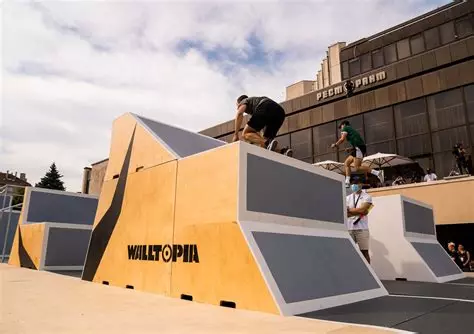
\includegraphics[width=0.50\textwidth]{terrain.png}
\end{frame}

\begin{frame}{Modèles}
\itemize{
	\item Les figures
	\item L'athlète
	\item Les cases
	\item Le terrain
	\item Algortihme Génétique
}
\end{frame}

\begin{frame}{Les résultats}
\begin{tabular}{lll}
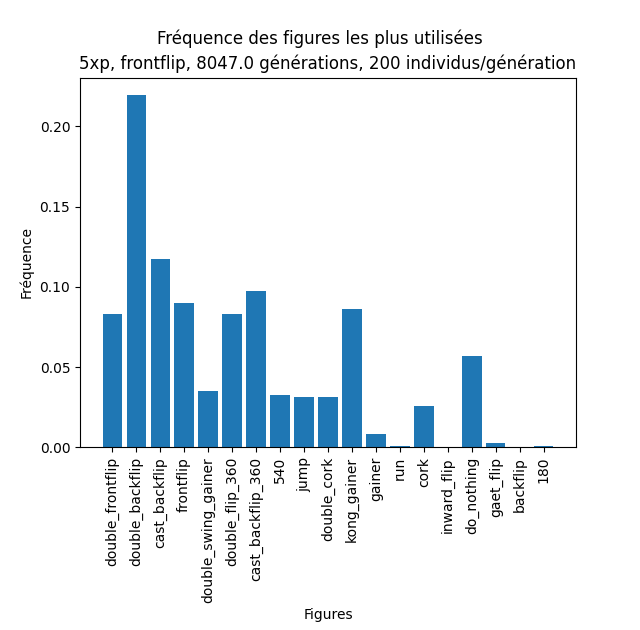
\includegraphics[width=0.25\textwidth]{15_fig_freq.png} & 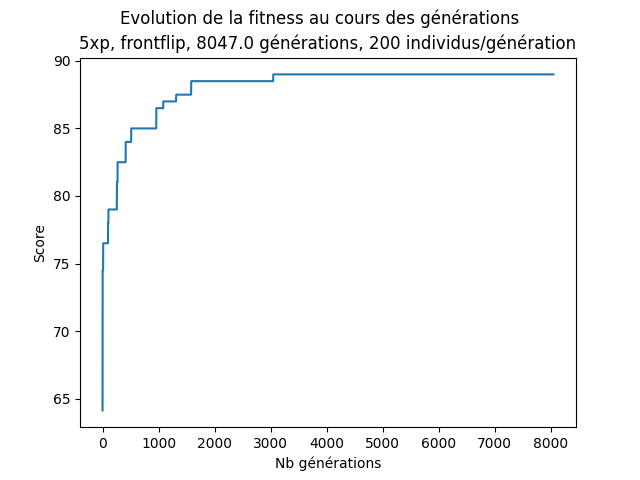
\includegraphics[width=0.30\textwidth]{15_fig_evol_fitness.png} &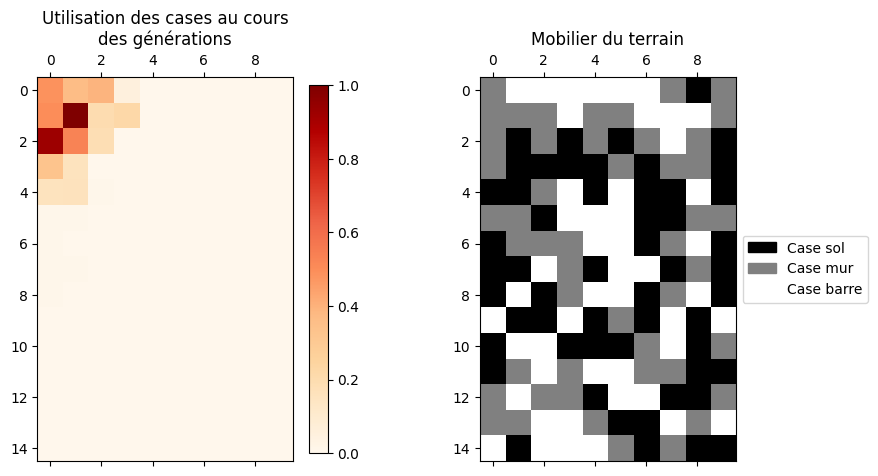
\includegraphics[width=0.40\textwidth]{15_fig_cases.png} \\
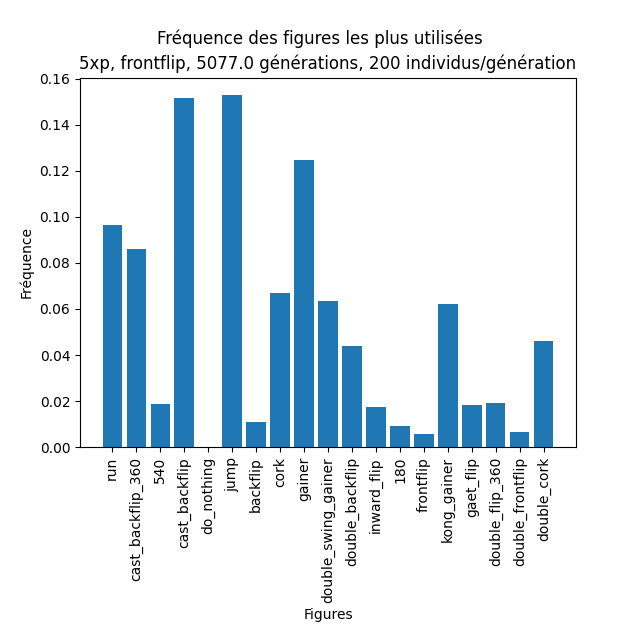
\includegraphics[width=0.25\textwidth]{nv_scoring_freq.png} & 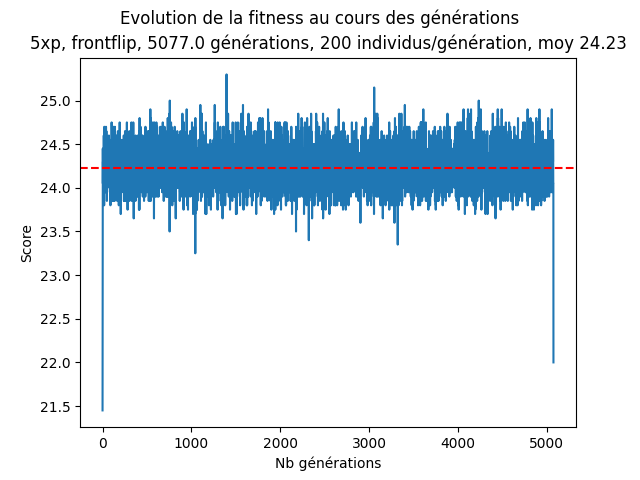
\includegraphics[width=0.30\textwidth]{nv_scoring_evol_fitness.png} & 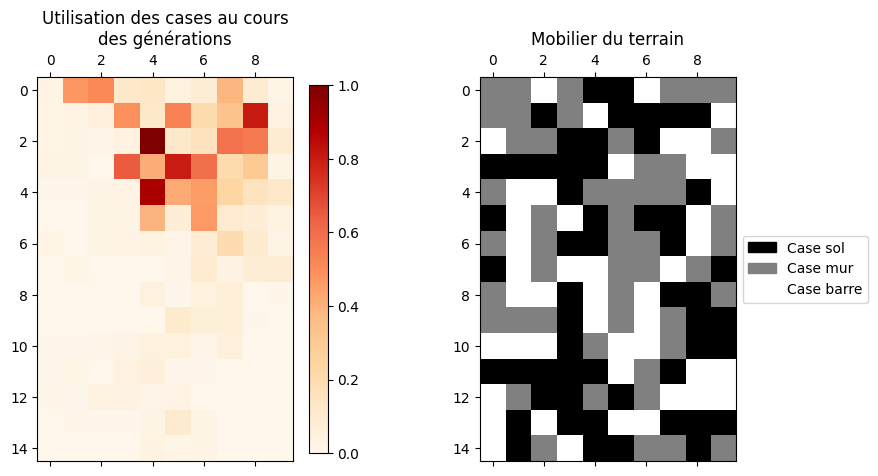
\includegraphics[width=0.40\textwidth]{nv_scoring_cases.png} \\
\end{tabular}
\end{frame}

\end{document}
